

\aula{02}{26}{agosto}{2026}

\begin{resposta}
    \begin{enumerate}[start=2]
        \item Determinação do carregamento nas lajes

        \begin{observacao}
            É preciso calcular o carregamento permanente para cada laje, mas como h = 10 cm para todos não precisou repetir.
        \end{observacao}

        \begin{figure}[H]
    \centering
    \begin{tikzpicture}[
    scale=1.5,
    cota/.style={<->, >=stealth, thin, black},
    chamada/.style={gray!80, thin},
    setaCarga/.style={->, >=stealth, black, thick},
    texto/.style={font=\small\sffamily}
]

    % --- Parâmetros de Geometria ---
    \def\vao{6.0}         % Comprimento do vão da laje
    \def\espPiso{0.25}    % Espessura da camada de piso
    \def\espLaje{0.80}    % Espessura da laje de concreto
    \def\espForro{0.15}   % Espessura da camada de forro

    % --- Coordenadas das Camadas (Origem na face inferior da laje) ---
    \coordinate (F_E_Inf) at (0, -\espForro);
    \coordinate (F_D_Sup) at (\vao, 0);
    
    \coordinate (L_E_Inf) at (0, 0);
    \coordinate (L_D_Sup) at (\vao, \espLaje);
    
    \coordinate (P_E_Inf) at (0, \espLaje);
    \coordinate (P_D_Sup) at (\vao, \espLaje + \espPiso);

    % --- 1. Camada de Forro / Acabamento Inferior ---
    \fill[gray!10!white] (F_E_Inf) rectangle (F_D_Sup);
    \draw[thick, black] (F_E_Inf) rectangle (F_D_Sup);

    % --- 2. Laje de Concreto Armado ---
    \fill[white] (L_E_Inf) rectangle (L_D_Sup);
    % Textura em hachura de concreto
    %\pattern[pattern=dots, pattern color=black!60] (L_E_Inf) rectangle (L_D_Sup);
    \draw[thick, black] (L_E_Inf) rectangle (L_D_Sup);

    % Representação das barras de armadura de aço (superior e inferior)
    %\draw[red!60!black, ultra thick] (0.2, 0.15) -- (\vao-0.2, 0.15);
    %\draw[red!60!black, ultra thick] (0.2, \espLaje-0.15) -- (\vao-0.2, \espLaje-0.15);

    % --- 3. Camada de Piso / Revestimento ---
    \fill[white] (P_E_Inf) rectangle (P_D_Sup);
    % Textura em hachura de concreto
    \pattern[pattern=vertical lines, pattern color=black!60]  (P_E_Inf) rectangle (P_D_Sup);
    \draw[thick, black] (P_E_Inf) rectangle (P_D_Sup);

    % --- Apóios da Laje nas extremidades (Vigas) ---
    %\draw[thick, fill=gray!50] (-0.5, -\espForro) rectangle (0, \espLaje);
    %\draw[thick, fill=gray!50] (\vao, -\espForro) rectangle (\vao+0.5, \espLaje);

    % --- 4. Carga de Uso Distribuída (Setas no Topo do Piso) ---
    \def\yPiso{\espLaje + \espPiso}
    \def\alturaSetas{0.7}
    \def\yTopoSetas{\yPiso + \alturaSetas}

    \draw[black, thick] (0, \yTopoSetas) -- (\vao, \yTopoSetas);

    \foreach \x in {0, 1, 2, 3, 4, 5, 6} {
        \draw[setaCarga] (\x, \yTopoSetas) -- (\x, \yPiso);
    }
    \node[texto, black, font=\bfseries\small, above] at (\vao/2, \yTopoSetas) {Carga de uso};

    % --- 5. Linhas de Chamada e Rótulos das Camadas ---
    \draw[chamada, ->, >=stealth] (\vao + 0.8, \yPiso - 0.12) -- (\vao - 0.5, \yPiso - 0.12);
    \node[texto, right] at (\vao + 0.8, \yPiso - 0.12) {Piso + Revestimento};

    \draw[chamada, ->, >=stealth] (\vao + 0.8, \espLaje/2) -- (\vao - 0.5, \espLaje/2);
    \node[texto, right] at (\vao + 0.8, \espLaje/2) {\begin{tabular}{l} Laje ($h=10\ cm$)) \end{tabular}};

    \draw[chamada, ->, >=stealth] (\vao + 0.8, -\espForro/2) -- (\vao - 0.5, -\espForro/2);
    \node[texto, right] at (\vao + 0.8, -\espForro/2) {Forro};

\end{tikzpicture}
    %\caption{Corte longitudinal da laje.}
    %\label{fig:corte-laje}
\end{figure}

        $g_{PP} = \gamma_{ap} \cdot h = 25 \times 10 \cdot 10^{-2} = 2,5 \ kN/m^2 \to \gamma_{ap}=25 \ kN/m^3$ \cite[tabela 1]{nbr6120}

        $g_{P+R} = 1 \ kN/m^2$ \cite[tabela 4]{nbr6120}

        $g_{forro}= 0,25 \ kN/m^2$ \cite[tabela 8]{nbr6120} \newline

        $g= g_{PP}+g_{P+R}+g_{forro} = 2,5+1+0,25=3,75 \ kN/m^2$

        $q= 3 \ kN/m^2$ \cite[tabela 10]{nbr6120} \newline

        $g+q=3,75+3=6,75\ kN/m^2$ \newline

        \item Vinculação das lajes

        \begin{observacao}
            Multiplica por três por causa da recomendação do livro IBRACON.
        \end{observacao}

        \fbox{L1}

            \begin{enumerate}
                \item Vizinhança V5

                \begin{figure}[H]
    \centering
\begin{tikzpicture}[
    scale=1.5,
    cota/.style={<->, >=stealth, thin, gray!80!black},  % Estilo das linhas de cota
    retangulo/.style={draw=gray!80!black, thick},        % Estilo do retângulo
    chamada/.style={gray!60, thin, dashed},              % Linhas de chamada/extensão
    eixo/.style={->, >=stealth, thick, gray!80!black}   % Estilo dos eixos x e y
]

    % --- Parâmetros de Dimensão ---
    \def\wE{2} % Largura do retângulo esquerdo
    \def\hE{1} % Altura do retângulo esquerdo
    
    \def\wD{1} % Largura do retângulo direito (menor)
    \def\hD{2} % Altura do retângulo direito (menor)
    
    % --- Coordenadas ---
    % Topo comum em y = \hE
    \coordinate (A_E) at (0, 0);                 % Canto inf. esq. do esquerdo
    \coordinate (B_E) at (\wE, 0);               % Canto inf. dir. do esquerdo
    \coordinate (C_E) at (\wE, \hE);             % Canto sup. dir. do esquerdo
    \coordinate (D_E) at (0, \hE);               % Canto sup. esq. do esquerdo

    \coordinate (A_D) at (\wE, \hE - \hD);       % Canto inf. esq. do direito
    \coordinate (B_D) at (\wE + \wD, \hE - \hD); % Canto inf. dir. do direito
    \coordinate (C_D) at (\wE + \wD, \hE);        % Canto sup. dir. do direito

    % --- 1. Desenho dos Retângulos (Alinhados no topo em y = \hE) ---
    \draw[retangulo] (A_E) rectangle (C_E); % Retângulo da esquerda
    \draw[retangulo] (A_D) rectangle (C_D); % Retângulo da direita
    \draw[retangulo, black, line width=3pt] (C_E) rectangle (B_E); 
    %\draw[retangulo, black, line width=3pt] (A_E) rectangle (B_E); 

    % --- 2. Números nos centros dos retângulos ---
    \node[font=\large\bfseries, gray!80!black] at ($(A_E)!0.5!(C_E)$) {L1};
    \node[font=\large\bfseries, gray!80!black] at ($(A_D)!0.5!(C_D)$) {L2};

    % --- 2. Eixos de Coordenadas x e y (Canto inf. esq. do retângulo da esquerda) ---
    %\draw[eixo] (0.2, 0.2) -- (0.8, 0.2) node[above, font=\small\bfseries] {$x$};
    %\draw[eixo] (0.2, 0.2) -- (0.2, 0.8) node[right, font=\small\bfseries] {$y$};

    % --- 3. Cotas Horizontais Inferiores (Eixo único com comprimentos separados) ---
    \def\offsetH{1.5} % Distância do nível inferior do retângulo da esquerda
    \def\yCota{-\offsetH}

    % Linhas de chamada verticais estendidas até a cota
    %\draw[chamada] (A_E) -- (0, \yCota - 0.15);
    %\draw[chamada] (B_E) -- (\wE, \yCota - 0.15);
    %\draw[chamada] (B_D) -- (\wE + \wD, \yCota - 0.15);

    % Cota do Retângulo da Esquerda (b1)
    \draw[cota] (0, \yCota) -- (\wE, \yCota) 
        node[midway, below=3pt, font=\small] {$476 \ \text{ cm}$};

    % Cota do Retângulo da Direita (b2)
    \draw[cota] (\wE, \yCota) -- (\wE + \wD, \yCota) 
        node[midway, below=3pt, font=\small] {$446 \ \text{ cm}$};

\end{tikzpicture}
    %\caption{Dois retângulos alinhados no topo com cotas separadas na base}
    %\label{fig:retangulos_alinhados}
\end{figure}
    
                $\ell_1 < 3\ell_2 \newline 476 < 3 \times 446 \newline 476 < 1338 \to$ ambas engastadas
                
                \item Vizinhança V2

                \begin{figure}[H]
    \centering
\begin{tikzpicture}[
    scale=1.5,
    cota/.style={<->, >=stealth, thin, gray!80!black},  % Estilo das linhas de cota
    retangulo/.style={draw=gray!80!black, thick},        % Estilo do retângulo
    chamada/.style={gray!60, thin, dashed},              % Linhas de chamada/extensão
    eixo/.style={->, >=stealth, thick, gray!80!black}   % Estilo dos eixos x e y
]

    % --- Parâmetros de Dimensão ---
    \def\wD{1} % Largura do retângulo superior (2)
    \def\hD{1.5} % Altura do retângulo superior (2)
    
    \def\wE{1} % Largura do retângulo inferior (1)
    \def\hE{2} % Altura do retângulo inferior (1)
    
    % --- Coordenadas ---
    % Retângulo 1 (Inferior)
    \coordinate (A1) at (0, 0);
    \coordinate (B1) at (\wE, 0);
    \coordinate (C1) at (\wE, \hE);
    \coordinate (D1) at (0, \hE);

    % Retângulo 2 (Superior, posicionado logo acima do retângulo 1)
    \coordinate (A2) at (0, \hE);
    \coordinate (B2) at (\wD, \hE);
    \coordinate (C2) at (\wD, \hE + \hD);
    \coordinate (D2) at (0, \hE + \hD);

    % --- 1. Desenho dos Retângulos ---
    \draw[retangulo] (A1) rectangle (C1); % Retângulo 1 (Inferior)
    \draw[retangulo] (A2) rectangle (C2); % Retângulo 2 (Superior)
    \draw[retangulo, black, line width=3pt] (C1) rectangle (D1); 

    % --- 2. Números nos centros dos retângulos ---
    \node[font=\large\bfseries, gray!80!black] at ($(A2)!0.5!(C2)$) {L1};
    \node[font=\large\bfseries, gray!80!black] at ($(A1)!0.5!(C1)$) {L4};

    % --- 3. Cotas Verticais (À esquerda, separadas para cada retângulo) ---
    \def\offsetV{0.5}
    \def\xCota{-\offsetV}

    % Linhas de chamada
    %\draw[chamada] (A1) -- (\xCota - 0.15, 0);
    %\draw[chamada] (D1) -- (\xCota - 0.15, \hE);
    %\draw[chamada] (D2) -- (\xCota - 0.15, \hE + \hD);

    % Altura do Retângulo 2
    \draw[cota] (\xCota, \hE) -- (\xCota, \hE + \hD)
        node[midway, left=3pt, font=\small, rotate=90, anchor=south] {$256\text{ cm}$};

    % Altura do Retângulo 1
    \draw[cota] (\xCota, 0) -- (\xCota, \hE)
        node[midway, left=3pt, font=\small, rotate=90, anchor=south] {$556\text{ cm}$};

\end{tikzpicture}
    %\caption{Dois retângulos empilhados com identificações e cotas}
    %\label{fig:retangulos_empilhados}
\end{figure}
    
                $\ell_1 < 3\ell_2 \newline 556 < 3 \times 256 \newline 556 < 768 \to$ ambas engastadas
                
            \end{enumerate}
    
            \fbox{L2}
    
            \begin{enumerate}
                \item Vizinhança V5

                \begin{figure}[H]
    \centering
\begin{tikzpicture}[
    scale=1.5,
    cota/.style={<->, >=stealth, thin, gray!80!black},  % Estilo das linhas de cota
    retangulo/.style={draw=gray!80!black, thick},        % Estilo do retângulo
    chamada/.style={gray!60, thin, dashed},              % Linhas de chamada/extensão
    eixo/.style={->, >=stealth, thick, gray!80!black}   % Estilo dos eixos x e y
]

    % --- Parâmetros de Dimensão ---
    \def\wE{1.5} % Largura do retângulo esquerdo
    \def\hE{1} % Altura do retângulo esquerdo
    
    \def\wD{1.5} % Largura do retângulo direito (menor)
    \def\hD{2} % Altura do retângulo direito (menor)
    
    % --- Coordenadas ---
    % Retângulo da Esquerda (L4) - Base em y = 0
    \coordinate (A_E) at (0, 0);                 % Canto inf. esq.
    \coordinate (B_E) at (\wE, 0);               % Canto inf. dir.
    \coordinate (C_E) at (\wE, \hE);             % Canto sup. dir.
    \coordinate (D_E) at (0, \hE);               % Canto sup. esq.

    % Retângulo da Direita (L2) - Alinhado na BASE em y = 0
    \coordinate (A_D) at (\wE, 0);               % Canto inf. esq.
    \coordinate (B_D) at (\wE + \wD, 0);         % Canto inf. dir.
    \coordinate (C_D) at (\wE + \wD, \hD);        % Canto sup. dir.
    \coordinate (D_D) at (\wE, \hD);             % Canto sup. esq.

    % --- 1. Desenho dos Retângulos (Alinhados no topo em y = \hE) ---
    \draw[retangulo] (A_E) rectangle (C_E); % Retângulo da esquerda
    \draw[retangulo] (A_D) rectangle (C_D); % Retângulo da direita
    \draw[retangulo, black, line width=3pt] (C_E) rectangle (B_E); 
    %\draw[retangulo, black, line width=3pt] (A_E) rectangle (B_E); 

    % --- 2. Números nos centros dos retângulos ---
    \node[font=\large\bfseries, gray!80!black] at ($(A_E)!0.5!(C_E)$) {L4};
    \node[font=\large\bfseries, gray!80!black] at ($(A_D)!0.5!(C_D)$) {L2};

    % --- 2. Eixos de Coordenadas x e y (Canto inf. esq. do retângulo da esquerda) ---
    %\draw[eixo] (0.2, 0.2) -- (0.8, 0.2) node[above, font=\small\bfseries] {$x$};
    %\draw[eixo] (0.2, 0.2) -- (0.2, 0.8) node[right, font=\small\bfseries] {$y$};

    % --- 3. Cotas Horizontais Inferiores (Eixo único com comprimentos separados) ---
    \def\offsetH{0.5} % Distância do nível inferior do retângulo da esquerda
    \def\yCota{-\offsetH}

    % Linhas de chamada verticais estendidas até a cota
    %\draw[chamada] (A_E) -- (0, \yCota - 0.15);
    %\draw[chamada] (B_E) -- (\wE, \yCota - 0.15);
    %\draw[chamada] (B_D) -- (\wE + \wD, \yCota - 0.15);

    % Cota do Retângulo da Esquerda (b1)
    \draw[cota] (0, \yCota) -- (\wE, \yCota) 
        node[midway, below=3pt, font=\small] {$476 \ \text{ cm}$};

    % Cota do Retângulo da Direita (b2)
    \draw[cota] (\wE, \yCota) -- (\wE + \wD, \yCota) 
        node[midway, below=3pt, font=\small] {$446 \ \text{ cm}$};

\end{tikzpicture}
    %\caption{Dois retângulos alinhados no topo com cotas separadas na base}
    %\label{fig:retangulos_alinhados}
\end{figure}
    
                $\ell_1 < 3\ell_2 \newline 476 < 3 \times 446 \newline 476 < 1138 \to$ ambas engastadas
                
            \end{enumerate}

            \newpage
    
            \fbox{L3}
    
            \begin{observacao}
                Por ser uma laje em balanço precisa de engaste.
            \end{observacao}
    
            \begin{enumerate}
                \item Vizinhança V4

                \begin{figure}[H]
    \centering
\begin{tikzpicture}[
    scale=1.5,
    cota/.style={<->, >=stealth, thin, gray!80!black},  % Estilo das linhas de cota
    retangulo/.style={draw=gray!80!black, thick},        % Estilo do retângulo
    chamada/.style={gray!60, thin, dashed},              % Linhas de chamada/extensão
    eixo/.style={->, >=stealth, thick, gray!80!black}   % Estilo dos eixos x e y
]

    % --- Parâmetros de Dimensão ---
    \def\wE{1} % Largura do retângulo esquerdo
    \def\hE{2} % Altura do retângulo esquerdo
    
    \def\wD{1.5} % Largura do retângulo direito (menor)
    \def\hD{2} % Altura do retângulo direito (menor)
    
    % --- Coordenadas ---
    % Topo comum em y = \hE
    \coordinate (A_E) at (0, 0);                 % Canto inf. esq. do esquerdo
    \coordinate (B_E) at (\wE, 0);               % Canto inf. dir. do esquerdo
    \coordinate (C_E) at (\wE, \hE);             % Canto sup. dir. do esquerdo
    \coordinate (D_E) at (0, \hE);               % Canto sup. esq. do esquerdo

    \coordinate (A_D) at (\wE, \hE - \hD);       % Canto inf. esq. do direito
    \coordinate (B_D) at (\wE + \wD, \hE - \hD); % Canto inf. dir. do direito
    \coordinate (C_D) at (\wE + \wD, \hE);        % Canto sup. dir. do direito

    % --- 1. Desenho dos Retângulos (Alinhados no topo em y = \hE) ---
    \draw[retangulo] (A_E) rectangle (C_E); % Retângulo da esquerda
    \draw[retangulo] (A_D) rectangle (C_D); % Retângulo da direita
    \draw[retangulo, black, line width=3pt] (C_E) rectangle (B_E); 
    \draw[retangulo, white, dashed] (A_E) rectangle (D_E); 
    %\draw[retangulo, black, line width=3pt] (A_E) rectangle (B_E); 

    % --- 2. Números nos centros dos retângulos ---
    \node[font=\large\bfseries, gray!80!black] at ($(A_E)!0.5!(C_E)$) {L3};
    \node[font=\large\bfseries, gray!80!black] at ($(A_D)!0.5!(C_D)$) {L4};

    % --- 2. Eixos de Coordenadas x e y (Canto inf. esq. do retângulo da esquerda) ---
    %\draw[eixo] (0.2, 0.2) -- (0.8, 0.2) node[above, font=\small\bfseries] {$x$};
    %\draw[eixo] (0.2, 0.2) -- (0.2, 0.8) node[right, font=\small\bfseries] {$y$};

    % --- 3. Cotas Horizontais Inferiores (Eixo único com comprimentos separados) ---
    \def\offsetH{0.5} % Distância do nível inferior do retângulo da esquerda
    \def\yCota{-\offsetH}

    % Linhas de chamada verticais estendidas até a cota
    %\draw[chamada] (A_E) -- (0, \yCota - 0.15);
    %\draw[chamada] (B_E) -- (\wE, \yCota - 0.15);
    %\draw[chamada] (B_D) -- (\wE + \wD, \yCota - 0.15);

    % Cota do Retângulo da Esquerda (b1)
    \draw[cota] (0, \yCota) -- (\wE, \yCota) 
        node[midway, below=3pt, font=\small] {$153 \ \text{ cm}$};

    % Cota do Retângulo da Direita (b2)
    \draw[cota] (\wE, \yCota) -- (\wE + \wD, \yCota) 
        node[midway, below=3pt, font=\small] {$476 \ \text{ cm}$};

\end{tikzpicture}
    %\caption{Dois retângulos alinhados no topo com cotas separadas na base}
    %\label{fig:retangulos_alinhados}
\end{figure}
    
                $\ell_1 < 3\ell_2 \newline 476 < 3 \times 153 \newline 476 < 459 \to$ ambas engastadas
    
            \begin{observacao}
                Maior laje fica apoiada e a menor fica engastada.
            \end{observacao}
                
            \end{enumerate}            
        %\end{enumerate}

        \item Reações verticais nas lajes

        \begin{enumerate}
            \item Charneiras plásticas

            \fbox{L1}
    
            \begin{figure}[H]
    \centering
\begin{tikzpicture}[
    scale=2,
    cota/.style={<->, >=stealth, thin, gray!80!black},
    retangulo/.style={draw=gray!80!black, thick},
    divisao/.style={draw=black, thick, dashed},          % Charneiras / linhas de divisão
    eixo/.style={->, >=stealth, thick, gray!80!black},
    corte/.style={draw=black, dash dot, thick},          % Linhas dos cortes A e B
    setaCorte/.style={->, >=stealth, thick, black}
]

    % 1. Coordenadas dos Vértices do Retângulo
    \coordinate (A) at (0, 0);     % Canto inferior esquerdo
    \coordinate (B) at (3, 0);     % Canto inferior direito
    \coordinate (C) at (3, 2);     % Canto superior direito
    \coordinate (D) at (0, 2);     % Canto superior esquerdo

    % Interseções internas das linhas de divisão (charneiras plásticas)
    \coordinate (P1) at (0.732, 1.268);
    \coordinate (P2) at (1.732, 1.268);

    % 2. Hachuras externas sem borda (Engastes: base e lateral direita)
    \path[pattern={Lines[angle=45, distance=6pt, line width=0.5pt]}, pattern color=gray!60] (0, -0.3) rectangle (3.3, 0);
    \path[pattern={Lines[angle=45, distance=6pt, line width=0.5pt]}, pattern color=gray!60] (3, 0) rectangle (3.3, 2);

    % 3. Desenho do Retângulo Principal
    \draw[retangulo] (A) rectangle (C);

    % 4. Linhas de Divisão de Carga (Charneiras)
    \draw[divisao] (A) -- (P1);
    \draw[divisao] (D) -- (P1);
    \draw[divisao] (P1) -- (P2);
    \draw[divisao] (B) -- (P2);
    \draw[divisao] (C) -- (P2);

    % 5. Linhas dos Cortes A-A e B-B
    % Corte A-A (Horizontal pelo centro em y = 1.0)
    \draw[corte] (-0.5, 1.0) -- (3.5, 1.0);
    \draw[setaCorte] (-0.5, 1.0) -- (-0.5, 1.3) node[above, font=\small\bfseries] {A};
    \draw[setaCorte] (3.5, 1.0) -- (3.5, 1.3) node[above, font=\small\bfseries] {A};

    % Corte B-B (Vertical pelo centro em x = 1.5)
    \draw[corte] (1.5, -0.7) -- (1.5, 2.5);
    \draw[setaCorte] (1.5, 2.5) -- (1.8, 2.5) node[right, font=\small\bfseries] {B};
    \draw[setaCorte] (1.5, -0.7) -- (1.8, -0.7) node[right, font=\small\bfseries] {B};

    % 6. Textos das divisões (1, 2, 3, 4)
    \node[font=\small\bfseries, gray!90!black, fill=white, inner sep=1.5pt, circle] at (0.35, 1.0) {$A_y$};
    \node[font=\small\bfseries, gray!90!black, fill=white, inner sep=1.5pt, circle] at (1.23, 1.6) {$A_x$};
    \node[font=\small\bfseries, gray!90!black, fill=white, inner sep=1.5pt, circle] at (2.4, 1.0) {$A'_y$};
    \node[font=\small\bfseries, gray!90!black, fill=white, inner sep=1.5pt, circle] at (1.23, 0.5) {$A'_x$};

    % 7. Arcos e Rótulos dos Ângulos
    % Canto A (inferior esquerdo) - 60°
    \draw[thin, gray!80!black] (0.6, 0) arc (0:60:0.6);
    \node[font=\tiny, gray!90!black] at (0.75, 0.3) {$60^\circ$};

    % Canto D (superior esquerdo) - 45° EM RELAÇÃO À BORDA ESQUERDA (VERTICAL)
    \draw[thin, gray!80!black] (0, 1.5) arc (270:315:0.5);
    \node[font=\tiny, gray!90!black] at (0.3, 1.45) {$45^\circ$};

    % Canto B (inferior direito) - 45°
    \draw[thin, gray!80!black] (2.5, 0) arc (180:135:0.5);
    \node[font=\tiny, gray!90!black] at (2.35, 0.25) {$45^\circ$};

    % Canto C (superior direito) - 60°
    \draw[thin, gray!80!black] (3, 1.5) arc (270:210:0.5);
    \node[font=\tiny, gray!90!black] at (2.7, 1.4) {$60^\circ$};

    % 8. Eixos de Coordenadas x e y
    \draw[eixo] (0.1, 0.1) -- (0.5, 0.1) node[above=-1pt, font=\tiny\bfseries] {$x$};
    \draw[eixo] (0.1, 0.1) -- (0.1, 0.5) node[right=-1pt, font=\tiny\bfseries] {$y$};

    % 9. Cotas de Dimensão
    %\def\offsetH{1.1}
    %%\draw[cota] (0, -\offsetH) -- (3, -\offsetH) 
     %   node[midway, below=3pt, font=\small] {$476\text{ cm}$};

    %\def\offsetV{0.8}
    %%\draw[cota] (-\offsetV, 0) -- (-\offsetV, 2) 
     %   node[midway, left=3pt, font=\small, rotate=90, anchor=south] {$256 \text{ cm}$};

\end{tikzpicture}
    %\caption{Divisão de áreas de carga de laje com linhas de corte A-A e B-B}
    %\label{fig:divisao_laje}
\end{figure} \newpage

            \begin{multicols}{2}

                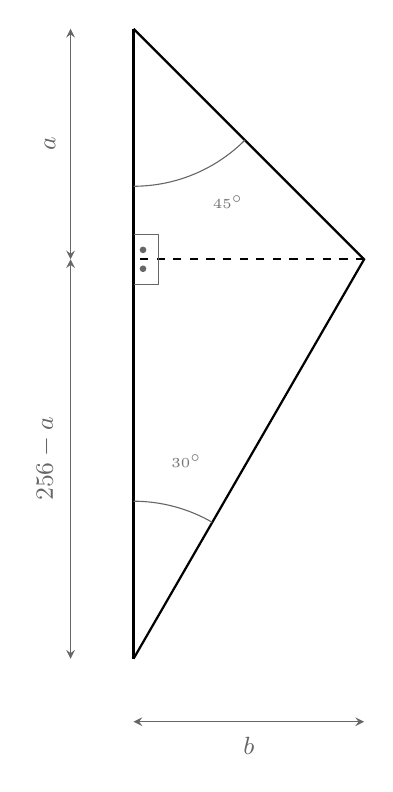
\begin{tikzpicture}[
    scale=4,
    cota/.style={<->, >=stealth, thin, gray!80!black},
    chamada/.style={gray!60, thin, dashed}
]
    % Coordenadas
    \coordinate (A) at (0, 0);
    \coordinate (D) at (0, 2);
    \coordinate (P1) at (0.732, 1.268);
    \coordinate (H) at (0, 1.268); % Ponto do corte na borda vertical

    % Desenho do Triângulo 1
    \draw[thick] (D) -- (A);                  % Borda livre da esquerda
    \draw[thick] (A) -- (P1) -- (D);          % Linhas de charneira
    \draw[thick,dashed] (P1) -- (H);          % Linha de corte/altura

    % Símbolos de Ângulo Reto (90°) na interseção da linha tracejada
    \draw[thin, gray!80!black] (0, 1.268-0.08) -- (0.08, 1.268-0.08) -- (0.08, 1.268);
    \fill[gray!80!black] (0.03, 1.268-0.03) circle (0.3pt);
    
    \draw[thin, gray!80!black] (0, 1.268+0.08) -- (0.08, 1.268+0.08) -- (0.08, 1.268);
    \fill[gray!80!black] (0.03, 1.268+0.03) circle (0.3pt);

    % Indicações dos Ângulos
    \draw[thin, gray!80!black] (0, 1.5) arc (270:315:0.5);
    \node[font=\tiny, gray!90!black] at (0.3, 1.45) {$45^\circ$};

    % Canto inferior (A): 30° da diagonal (60°) até a reta vertical (90°)
    \draw[thin, gray!80!black] (60:0.5) arc (60:90:0.5);
    \node[font=\tiny, gray!90!black] at (75:0.65) {$30^\circ$};

    % --- EIXO DE COTA HORIZONTAL (Largura x1) ---
    \def\offsetH{0.2}
    %\draw[chamada] (A) -- (0, -\offsetH);
    %\draw[chamada] (P1) -- (0.732, -\offsetH);
    \draw[cota] (0, -\offsetH) -- (0.732, -\offsetH)
        node[midway, below=2pt, font=\small] {$b$};

    % --- EIXOS DE COTA VERTICAIS (Alturas) ---
    \def\offsetV{0.2}
    %\draw[chamada] (A) -- (-\offsetV, 0);
    %\draw[chamada] (H) -- (-\offsetV, 1.268);
    %\draw[chamada] (D) -- (-\offsetV, 2);

    % Altura do trecho inferior
    \draw[cota] (-\offsetV, 0) -- (-\offsetV, 1.268)
        node[midway, left=2pt, font=\small, rotate=90, anchor=south] {$256-a$};

    % Altura do trecho superior
    \draw[cota] (-\offsetV, 1.268) -- (-\offsetV, 2)
        node[midway, left=2pt, font=\small, rotate=90, anchor=south] {$a$};

\end{tikzpicture}
    
                $\cancelto{1}{\tan 45}=\frac{b}{a} \longleftrightarrow b=a$ \newline
    
                $\tan 30=\frac{a}{256-a} \newline \frac{\sqrt{3}}{3} (256-a)=a \newline \frac{256\sqrt{3}}{3}=(1+\frac{\sqrt{3}}{3})a \newline a \approx 93,70 \ cm$ \newline
    
                $L=256-a\newline L\approx256-93,70 \newline L\approx 162,30 \ cm$ \newline
            \end{multicols}

            $A_y= \frac{bh}{2}\approx\frac{256\times 93,7}{2}\approx1,2 \ m^2$ \newline

            $V_y = \frac{(g+q)A_y}{\ell_x}\approx\frac{6,75 \times 1,2}{2,56}\approx3,16 \ kN/m$ \newline

            \begin{multicols}{2}

                \begin{tikzpicture}[
    scale=3,
    cota/.style={<->, >=stealth, thin, gray!80!black},
    chamada/.style={gray!60, thin, dashed}
]
    % Coordenadas espelhadas na vertical
    \coordinate (A) at (1.268, 0);
    \coordinate (D) at (1.268, 2);
    \coordinate (P1) at (0, 1.268);
    \coordinate (H) at (1.268, 1.268); % Ponto do corte na borda direita

    % Desenho do Triângulo
    \draw[thick] (D) -- (A);                  % Borda vertical da direita
    \draw[thick] (A) -- (P1) -- (D);          % Linhas de charneira
    \draw[thick,dashed] (P1) -- (H);          % Linha de corte/altura

    % Símbolos de Ângulo Reto (90°) na interseção
    \draw[thin, gray!80!black] (1.268, 1.268-0.08) -- (1.268-0.08, 1.268-0.08) -- (1.268-0.08, 1.268);
    \fill[gray!80!black] (1.268-0.03, 1.268-0.03) circle (0.3pt);
    
    \draw[thin, gray!80!black] (1.268, 1.268+0.08) -- (1.268-0.08, 1.268+0.08) -- (1.268-0.08, 1.268);
    \fill[gray!80!black] (1.268-0.03, 1.268+0.03) circle (0.3pt);

    % --- INDICAÇÃO DOS ÂNGULOS ---
    % Canto superior (D): 60° com a vertical
    \draw[thin, gray!80!black] (1.268, 1.5) arc (270:210:0.5);
    \node[font=\tiny, gray!90!black] at (1.268-0.35, 1.55) {$60^\circ$};

    % Canto inferior (A): 45° com a vertical
    \draw[thin, gray!80!black] ($(A)+(135:0.5)$) arc (135:90:0.5);
    \node[font=\tiny, gray!90!black] at (1.268-0.25, 0.5) {$45^\circ$};

    % --- EIXO DE COTA HORIZONTAL (Largura c) ---
    \def\offsetH{0.2}
    %\draw[chamada] (A) -- (1.268, -\offsetH);
    %\draw[chamada] (P1) -- (0, -\offsetH);
    \draw[cota] (0, -\offsetH) -- (1.268, -\offsetH)
        node[midway, below=2pt, font=\small] {$c$};

    % --- EIXOS DE COTA VERTICAIS (Alturas à direita) ---
    \def\offsetV{0.2}
    %\draw[chamada] (A) -- (1.268+\offsetV, 0);
    %\draw[chamada] (H) -- (1.268+\offsetV, 1.268);
    %\draw[chamada] (D) -- (1.268+\offsetV, 2);

    \draw[cota] (1.268+\offsetV, 0) -- (1.268+\offsetV, 1.268)
        node[midway, right=2pt, font=\small, rotate=-90, anchor=south] {$c$};

    \draw[cota] (1.268+\offsetV, 1.268) -- (1.268+\offsetV, 2)
        node[midway, right=2pt, font=\small, rotate=-90, anchor=south] {$256-c$};

\end{tikzpicture}

                $\tan 60 =\frac{c}{256-c} \newline 256 \sqrt{3}=(1+\sqrt{3})c \newline c \approx 162,30 \ cm$ \newline
    
                $L=256-c\newline\approx256-162,30\newline \approx93,70 \ cm$ \newline
                
            \end{multicols}

            $A'_y=\frac{bh}{2}\approx\frac{256\times162,30}{2}\approx2,08 \ m^2$ \newline

            $V'_y=\frac{(g+q)A'_y}{\ell_x}=\frac{6,75\times 2,08}{2,56} \approx5,48 \ kN/m$ \newline

            %\begin{multicols}{2}
            %\end{multicols}

            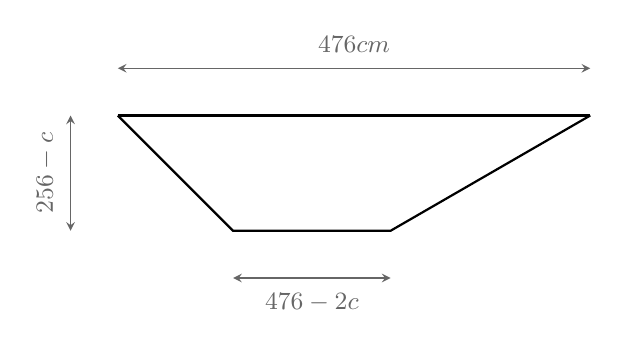
\begin{tikzpicture}[
    scale=2,
    cota/.style={<->, >=stealth, thin, gray!80!black},
    chamada/.style={gray!60, thin, dashed}
]
    % Coordenadas
    \coordinate (D) at (0, 2);
    \coordinate (C) at (3, 2);
    \coordinate (P1) at (0.732, 1.268);
    \coordinate (P2) at (1.732, 1.268);

    % Desenho do Trapézio 2
    \draw[thick] (D) -- (C);                         % Borda livre superior
    \draw[thick] (D) -- (P1) -- (P2) -- (C);         % Linhas de charneira

    % --- EIXO DE COTA HORIZONTAL SUPERIOR (Base Maior) ---
    \def\offsetHTopo{0.3}
    %\draw[chamada] (D) -- (0, 2 + \offsetHTopo + 0.05);
    %\draw[chamada] (C) -- (3, 2 + \offsetHTopo + 0.05);
    \draw[cota] (0, 2 + \offsetHTopo) -- (3, 2 + \offsetHTopo)
        node[midway, above=2pt, font=\small] {$476\text{ cm}$};

    % --- EIXOS DE COTA HORIZONTAIS INFERIORES (Base Menor e Projeções) ---
    \def\offsetHBaixo{0.3}
    \def\yCotaBaixo{1.268 - \offsetHBaixo}

    %\draw[chamada] (0, 1.268) -- (0, \yCotaBaixo - 0.05);
    %\draw[chamada] (P1) -- (0.732, \yCotaBaixo - 0.05);
    %\draw[chamada] (P2) -- (1.732, \yCotaBaixo - 0.05);
    %\draw[chamada] (3, 1.268) -- (3, \yCotaBaixo - 0.05);

    % Trecho esquerdo
    %\draw[cota] (0, \yCotaBaixo) -- (0.732, \yCotaBaixo)
     %   node[midway, below=2pt, font=\small] {$c$};

    % Base menor
    \draw[cota] (0.732, \yCotaBaixo) -- (1.732, \yCotaBaixo)
        node[midway, below=2pt, font=\small] {$476 - 2c$};

    % Trecho direito
    %\draw[cota] (1.732, \yCotaBaixo) -- (3, \yCotaBaixo)
     %   node[midway, below=2pt, font=\small] {$c$};

    % --- EIXO DE COTA VERTICAL (Altura do Trapézio) ---
    \def\offsetV{0.3}
    %\draw[chamada] (D) -- (-\offsetV - 0.05, 2);
    %\draw[chamada] (0, 1.268) -- (-\offsetV - 0.05, 1.268);
    \draw[cota] (-\offsetV, 1.268) -- (-\offsetV, 2)
        node[midway, left=2pt, font=\small, rotate=90, anchor=south] {$256-c$};

\end{tikzpicture}

            $b=476-2c\approx476-93,7-162,3=220 \ cm$ \newline

            $A_x=\frac{(B+b)h}{2}\approx\frac{(476+220)93,7}{2}\approx3,26 \ m^2$ \newline

            $V_x=\frac{(g+q)A_x}{\ell_y}\approx\frac{6,75\times 3,26}{4,76}\approx4,62 \ kN/m$ \newline

            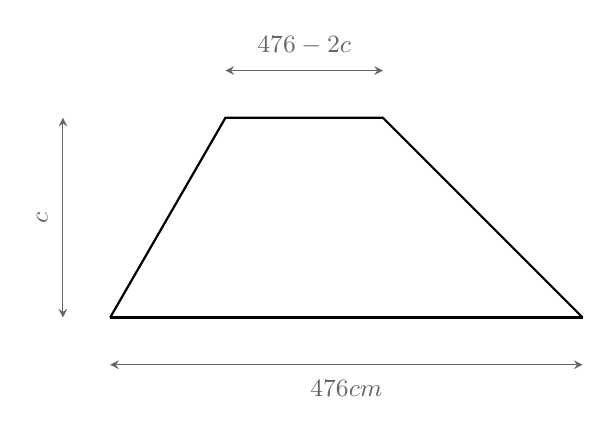
\begin{tikzpicture}[
    scale=2,
    cota/.style={<->, >=stealth, thin, gray!80!black},
    chamada/.style={gray!60, thin, dashed}
]
    % Coordenadas
    \coordinate (A) at (0, 0);
    \coordinate (B) at (3, 0);
    \coordinate (P1) at (0.732, 1.268);
    \coordinate (P2) at (1.732, 1.268);

    % Hachura do Engaste na base
    %\path[pattern={Lines[angle=45, distance=6pt, line width=0.5pt]}, pattern color=gray!60] (0, -0.3) rectangle (3, 0);

    % Desenho do Trapézio 4
    \draw[thick] (A) -- (B);                         % Borda engastada
    \draw[thick] (A) -- (P1) -- (P2) -- (B); % Linhas de charneira

    % Rótulo da Região
    %\node[font=\small\bfseries, gray!90!black, fill=white, inner sep=1.5pt, circle] at (1.232, 0.5) {4};

    % --- EIXO DE COTA HORIZONTAL INFERIOR (Base Maior - abaixo do engaste) ---
    \def\offsetHBaixo{0.3}
    %\draw[chamada] (A) -- (0, -\offsetHBaixo - 0.05);
    %\draw[chamada] (B) -- (3, -\offsetHBaixo - 0.05);
    \draw[cota] (0, -\offsetHBaixo) -- (3, -\offsetHBaixo)
        node[midway, below=2pt, font=\small] {$476\text{ cm}$};

    % --- EIXOS DE COTA HORIZONTAIS SUPERIORES (Base Menor e Projeções) ---
    \def\offsetHTopo{0.3}
    \def\yCotaTopo{1.268 + \offsetHTopo}

    %\draw[chamada] (0, 0) -- (0, \yCotaTopo + 0.05);
    %\draw[chamada] (P1) -- (0.732, \yCotaTopo + 0.05);
    %\draw[chamada] (P2) -- (1.732, \yCotaTopo + 0.05);
    %\draw[chamada] (3, 0) -- (3, \yCotaTopo + 0.05);

    % Projeção esquerda
    %\draw[cota] (0, \yCotaTopo) -- (0.732, \yCotaTopo)
        %node[midway, above=2pt, font=\small] {$c$};

    % Base menor
    \draw[cota] (0.732, \yCotaTopo) -- (1.732, \yCotaTopo)
        node[midway, above=2pt, font=\small] {$476 - 2c$};

    % Projeção direita
    %\draw[cota] (1.732, \yCotaTopo) -- (3, \yCotaTopo)
        %node[midway, above=2pt, font=\small] {$c$};

    % --- EIXO DE COTA VERTICAL (Altura do Trapézio) ---
    \def\offsetV{0.3}
    %\draw[chamada] (A) -- (-\offsetV - 0.05, 0);
    %\draw[chamada] (0, 1.268) -- (-\offsetV - 0.05, 1.268);
    \draw[cota] (-\offsetV, 0) -- (-\offsetV, 1.268)
        node[midway, left=2pt, font=\small, rotate=90, anchor=south] {$c$};

\end{tikzpicture}

            $A'_x=\frac{(B+b)h}{2}\approx\frac{(476+220)162,3}{2}\approx6,65 \ m^2$ \newline

            $V'_x=\frac{(g+q)A_x}{\ell_y}\approx\frac{6,75\times 5,65}{4,76}\approx8,01 \ kN/m$ \newline

            \paracasa

            \fbox{L2}

            \fbox{L3}

            \begin{figure}[H]
    \centering
\begin{tikzpicture}[
    scale=1.5,
    cota/.style={<->, >=stealth, thin, gray!80!black},  % Estilo das linhas de cota
    retangulo/.style={draw=gray!80!black, thick},        % Estilo do retângulo
    divisao/.style={draw=black, thick, dashed},          % Linhas de divisão (charneiras)
    eixo/.style={->, >=stealth, thick, gray!80!black},
    corte/.style={draw=black, dash dot, thick},          % Linhas dos cortes A e B
    setaCorte/.style={->, >=stealth, thick, black}
]

    % 1. Coordenadas do retângulo
    \coordinate (A) at (0, 0);
    \coordinate (B) at (2, 0);
    \coordinate (C) at (2, 4);
    \coordinate (D) at (0, 4);

    % Interseção P da charneira (ponto de encontro dos ângulos de 60°)
    % Forma um triângulo à direita e um trapézio à esquerda
    \coordinate (P1) at (0, 1.5);
    \coordinate (P2) at (0, 2.5);

    % 2. Hachuras externas no topo e na direita (sem borda)
    %\path[pattern={Lines[angle=45, distance=6pt, line width=0.5pt]}, pattern color=gray!60] (0, 3) rectangle (2.3, 3.3);
    \path[pattern={Lines[angle=45, distance=6pt, line width=0.5pt]}, pattern color=gray!60] (2, 0) rectangle (2.3, 4);

    % 3. Desenho do Retângulo
    \draw[retangulo] (A) rectangle (C);

    % 4. Divisão em Triângulo (direita) e Trapézio (esquerda)
    \draw[divisao] (C) -- (P2) --(P1) -- (B);

    % 5. Linhas dos Cortes A (Horizontal) e B (Vertical)
    % Corte A (Horizontal em y = 1.5)
    \draw[corte] (-0.4, 2) -- (2.5, 2);
    \draw[setaCorte] (-0.4, 2) -- (-0.4, 2.25) node[above, font=\small\bfseries] {A};
    \draw[setaCorte] (2.5, 2) -- (2.5, 2.25) node[above, font=\small\bfseries] {A};

    % Corte B (Vertical em x = 1.0)
    \draw[corte] (1.0, -0.6) -- (1.0, 4.5);
    \draw[setaCorte] (1.0, 4.5) -- (1.3,4.5) node[right, font=\small\bfseries] {B};
    \draw[setaCorte] (1.0, -0.6) -- (1.3, -0.6) node[right, font=\small\bfseries] {B};
    
    \node[font=\small\bfseries, gray!90!black, fill=white, inner sep=1.5pt, circle] at (0.5, 3.5) {$A_y$};
    %\node[font=\small\bfseries, gray!90!black, fill=white, inner sep=1.5pt, circle] at (1.23, 1.6) {$A_x$};
    \node[font=\small\bfseries, gray!90!black, fill=white, inner sep=1.5pt, circle] at (0.5, 0.5) {$A_y$};
    \node[font=\small\bfseries, gray!90!black, fill=white, inner sep=1.5pt, circle] at (1, 2) {$A'_x$};

    % 6. Indicações dos Ângulos de 60° na borda direita
    % Canto superior direito (C): 60° em relação à borda vertical
    \draw[thin, gray!80!black] (2, 3.3) arc (270:210:0.7);
    \node[font=\tiny, gray!90!black] at (1.75, 3.2) {$60^\circ$};

    % Canto inferior direito (B): 60° em relação à borda vertical
    \draw[thin, gray!80!black] (2, 0.7) arc (90:150:0.7);
    \node[font=\tiny, gray!90!black] at (1.75, 0.8) {$60^\circ$};

    % 7. Eixos de Coordenadas x e y
    \draw[eixo] (0.2, 0.2) -- (0.7, 0.2) node[above=-2pt, font=\tiny\bfseries] {$x$};
    \draw[eixo] (0.2, 0.2) -- (0.2, 0.7) node[right=-2pt, font=\tiny\bfseries] {$y$};

    % 8. Cotas de Dimensão
    %\def\offsetH{0.4}
    %\draw[cota] (0, -\offsetH) -- (2, -\offsetH) 
        %node[midway, below=3pt, font=\small] {$476\text{ cm}$};

    %\def\offsetV{0.4}
    %\draw[cota] (-\offsetV, 0) -- (-\offsetV, 3) 
        %node[midway, left=3pt, font=\small, rotate=90, anchor=south] {$556 \text{ cm}$};

\end{tikzpicture}
    %\caption{Retângulo dividido em triângulo e trapézio com cortes A e B}
    %\label{fig:retangulo_triangulo_trapezio}
\end{figure}

            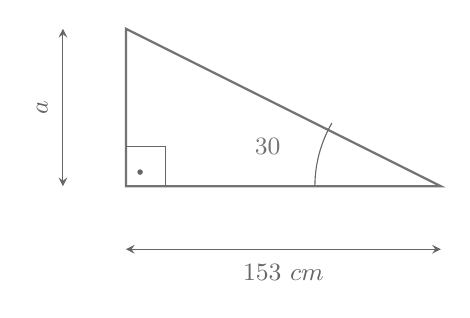
\begin{tikzpicture}[
    scale=2,
    cota/.style={<->, >=stealth, thin, gray!80!black},
    chamada/.style={gray!60, thin, dashed}
]
    % 1. Coordenadas dos vértices (Triângulo Retângulo 3-4-5)
    \coordinate (A) at (0,0); % Canto do ângulo reto
    \coordinate (B) at (2,0); % Canto inferior direito
    \coordinate (C) at (0,1); % Canto superior esquerdo

    % 2. Desenho do Triângulo
    \draw[thick, gray!90!black] (A) -- (B) -- (C) -- cycle;

    % 3. Símbolo de Ângulo Reto (90°)
    \draw[thin, gray!80!black] (0, 0.25) -- (0.25, 0.25) -- (0.25, 0);
    \fill[gray!80!black] (0.09, 0.09) circle (0.5pt);

    % 4. Indicação do Ângulo Theta em B
    \draw[thin, gray!80!black] (1.2, 0) arc (180:149.9:0.8);
    \node[font=\small, gray!90!black] at (0.9, 0.25) {$30$};

    % --- COTAS DE TAMANHO ---
    % Base (Cateto b)
    \def\offsetH{0.4}
    %\draw[chamada] (A) -- (0, -\offsetH - 0.05);
    %\draw[chamada] (B) -- (4, -\offsetH - 0.05);
    \draw[cota] (0, -\offsetH) -- (2, -\offsetH)
        node[midway, below=2pt, font=\small] {$153 \  \text{ cm}$};

    % Altura (Cateto a)
    \def\offsetV{0.4}
    %\draw[chamada] (A) -- (-\offsetV - 0.05, 0);
    %\draw[chamada] (C) -- (-\offsetV - 0.05, 3);
    \draw[cota] (-\offsetV, 0) -- (-\offsetV, 1)
        node[midway, left=2pt, font=\small, rotate=90, anchor=south] {$a$};

    % Hipotenusa (c) - Cota inclinada e paralela
    %\def\offsetHip{0.4}
    %\coordinate (B_cota) at ($(B) + (36.87:\offsetHip)$);
    %\coordinate (C_cota) at ($(C) + (36.87:\offsetHip)$);

    %\draw[chamada] (B) -- ($(B) + (36.87:\offsetHip + 0.05)$);
    %\draw[chamada] (C) -- ($(C) + (36.87:\offsetHip + 0.05)$);
    %\draw[cota] (B_cota) -- (C_cota)
        %node[midway, above right=-1pt, font=\small, rotate=-36.87] {$c = 5\text{ cm}$};

\end{tikzpicture}

            $\tan 30 = \frac{a}{1,53} \newline a\approx0,88 \ m$ \newline

            $A_y=\frac{bh}{2}\approx\frac{1,53\times0,88}{2}\approx0,68\ m^2$ \newline

            $V_y=\frac{(g+q)A_y}{\ell_x}\approx\frac{6,75\times0,68}{1,53}\approx2,98\ kN/m$ \newline

            \begin{figure}[H]
    \centering
\begin{tikzpicture}[
    scale=1.5,
    cota/.style={<->, >=stealth, thin, gray!80!black},
    chamada/.style={gray!60, thin, dashed},
    seta/.style={->, >=stealth, thick},
    cargaDist/.style={->, >=stealth, thin, black}
]

    % --- Parâmetros ---
    \def\L{4.0}       % Comprimento da viga (lx)
    \def\hArm{1.1}    % Altura do braço na ponta em balanço
    \def\qHeight{0.6} % Altura da representação da carga distribuída

    % --- Coordenadas principais ---
    \coordinate (A) at (0, 0);          % Extremidade livre (ponta em balanço)
    \coordinate (B) at (\L, 0);         % Engaste (direita)
    \coordinate (ArmTop) at (0, \hArm); % Topo do braço vertical de altura 1,1

    % 1. Desenho do Corpo da Viga
    \draw[line width=3pt, gray!80!black] (A) -- (B);

    % 2. Engaste na Direita (Parede Hachurada em x = lx)
    \draw[thick] (\L, -0.8) -- (\L, 0.8);
    \path[pattern={Lines[angle=45, distance=5pt, line width=0.5pt]}, pattern color=gray!60] 
        (\L, -0.8) rectangle (\L + 0.3, 0.8);

    % 3. Haste/Braço Vertical na Ponta em Balanço (Altura 1,1)
    %\draw[line width=2pt, gray!80!black] (A) -- (ArmTop);

    % 4. Carga Distribuída Uniforme (q)
    \draw[thick, black] (0, \qHeight) -- (\L, \qHeight);
    \node[above, font=\small, black] at (\L/2, \qHeight) {$g+q$};
    \foreach \x in {0, 0.5, ..., \L} {
        \draw[cargaDist] (\x, \qHeight) -- (\x, 0.05);
    }

    % 5. Cargas Verticais na Ponta em Balanço
    \draw[seta, black, line width=1.2pt] (0, 2.25) -- (0, 1.25)  
        node[above left, font=\small] {$q_v$};
    \draw[seta, black, line width=1.2pt] (0, \hArm) -- (0, 0) 
        node[above left, font=\small] {$q_m$};

    % 6. Carga Horizontal a 1,1 de Altura
    \draw[seta, black, line width=1.2pt] (1.05, \hArm) -- (0.05, \hArm) 
        node[midway, above, font=\small] {$q_h$};

    % 7. Força Vertical V no Engaste
    \draw[seta, black, line width=1.2pt] (\L, -0.8) -- (\L, -0.05) 
        node[midway, right, font=\small] {$V'_x$};

    % 8. Cotas de Dimensão
    % Cota de Altura (1,1)
    \def\offsetArm{0.5}
    %\draw[chamada] (0, 0) -- (-\offsetArm, 0);
    %\draw[chamada] (0, \hArm) -- (-\offsetArm, \hArm);
    \draw[cota] (-\offsetArm, 0) -- (-\offsetArm, \hArm)
        node[midway, left=2pt, font=\small] {$1{,}1 \ m$};

    % Cota de Comprimento (lx)
    \def\offsetL{1.2}
    %\draw[chamada] (0, 0) -- (0, -\offsetL);
    %\draw[chamada] (\L, 0) -- (\L, -\offsetL);
    \draw[cota] (0, -\offsetL) -- (\L, -\offsetL)
        node[midway, below=2pt, font=\small] {$l_x$};

\end{tikzpicture}
    \caption{Corte AA.}
    \label{fig:viga_engastada}
\end{figure}

            $g_m = 1 \ kN/m$ Valor estimado da mureta \cite[item 6.3]{nbr6120} 

            $q_v = 2 \ kN/m$ carga acidental \cite[tabela 10, índice j]{nbr6120} 

            $q_h = 1 \ kN/m$ \cite[tabela 12]{nbr6120} \newline

            $V'_x=(g+q)\ell_x+g_m+q\to g_m=1,1 \ h_m\newline V'_x\approx6,75\times1,53+1,1\times 1 +2\newline V'_x\approx13,43\ kN/m$ \newline

            \fbox{L4}

            \item Método tabelado

            \fbox{L1}
    
            \begin{figure}[H]
    \centering
\begin{tikzpicture}[
    scale=1.5,
    cota/.style={<->, >=stealth, thin, gray!80!black},  % Estilo das linhas de cota
    retangulo/.style={draw=gray!80!black, thick},        % Estilo do retângulo
    eixo/.style={->, >=stealth, thick, gray!80!black}   % Estilo dos eixos x e y
]

    % 1. Coordenadas do retângulo
    \coordinate (A) at (0, 0);
    \coordinate (B) at (3, 0);
    \coordinate (C) at (3, 2);
    \coordinate (D) at (0, 2);

    % 2. Hachura horizontal sem borda DO LADO DE FORA (canto inferior e direito)
    % Faixa externa inferior (abaixo da base: y de -0.3 a 0)
    \path[pattern={Lines[angle=45, distance=6pt, line width=0.5pt]}, pattern color=gray!60] (0, -0.3) rectangle (3.3, 0);
    % Faixa externa lateral direita (à direita da borda: x de 3 a 3.3)
    \path[pattern={Lines[angle=45, distance=6pt, line width=0.5pt]}, pattern color=gray!60] (3, 0) rectangle (3.3, 2);

    % 3. Desenho do Retângulo
    \draw[retangulo] (A) rectangle (C);

    % 4. Eixos de Coordenadas x e y (Origem no canto inferior esquerdo, dentro do retângulo)
    \draw[eixo] (0.2, 0.2) -- (0.8, 0.2) node[above, font=\small\bfseries] {$y$};
    \draw[eixo] (0.2, 0.2) -- (0.2, 0.8) node[right, font=\small\bfseries] {$x$};

    % --- COTA HORIZONTAL (Afastada ligeiramente para não sobrepor a hachura) ---
    \def\offsetH{0.5}
    \draw[cota] (0, -\offsetH) -- (3, -\offsetH) 
        node[midway, below=3pt, font=\small] {$476\text{ cm}$};

    % --- COTA VERTICAL ---
    \def\offsetV{0.4}
    \draw[cota] (-\offsetV, 0) -- (-\offsetV, 2) 
        node[midway, left=3pt, font=\small, rotate=90, anchor=south] {$256 \text{ cm}$};

\end{tikzpicture}
    %\caption{Caption}
    %\label{fig:placeholder}
\end{figure}

            Laje tipo 3 \cite[tabela 2.2b]{tabelalajes}

            Por interpolação linear:

            \begin{table}[h]
                \centering
                \color{gray!80!black} 
                \begin{tabular}{l l l l l}
                    $\lambda$ & $v_x$ & $v'_x$ & $v_y$ & $v'_y$ \\
                    1,86 & 3,17 & 4,64 & 2,17 & 2,17
                \end{tabular}
                %\caption{Caption}
                %\label{tab:placeholder}
            \end{table}

            $V_x = v_x(g+q)\frac{l_x}{10}= 3,17 (6,75) \frac{2,56}{10}= 5,47 \ kN/m$

            $V'_x = v'_x(g+q)\frac{l_x}{10}= 8,01 \ kN/m$

            $V_y = v_y(g+q)\frac{l_x}{10}= 3,75 \ kN/m$

            $V'_y = v'_y(g+q)\frac{l_x}{10}= 5,48 \ kN/m$
    
            \fbox{L2}
    
            \begin{figure}[H]
    \centering
\begin{tikzpicture}[
    scale=1.5,
    cota/.style={<->, >=stealth, thin, gray!80!black},  % Estilo das linhas de cota
    retangulo/.style={draw=gray!80!black, thick},        % Estilo do retângulo
    eixo/.style={->, >=stealth, thick, gray!80!black}   % Estilo dos eixos x e y
]

    % 1. Coordenadas do retângulo
    \coordinate (A) at (0, 0);
    \coordinate (B) at (2, 0);
    \coordinate (C) at (2, 3);
    \coordinate (D) at (0, 3);

    % 2. Hachura no lado esquerdo (fora do retângulo, sem borda)
    % Vai de x = -0.3 até 0, ao longo de toda a altura (y = 0 até 3)
    \path[pattern={Lines[angle=45, distance=6pt, line width=0.5pt]}, pattern color=gray!60] (-0.3, 0) rectangle (0, 3);

    % 3. Desenho do Retângulo
    \draw[retangulo] (A) rectangle (C);

    % 4. Eixos de Coordenadas x e y (Origem no canto inferior esquerdo, dentro do retângulo)
    \draw[eixo] (0.2, 0.2) -- (0.8, 0.2) node[above, font=\small\bfseries] {$x$};
    \draw[eixo] (0.2, 0.2) -- (0.2, 0.8) node[right, font=\small\bfseries] {$y$};

    % --- COTA HORIZONTAL (Texto abaixo da linha) ---
    \def\offsetH{0.4}
    \draw[cota] (0, -\offsetH) -- (2, -\offsetH) 
        node[midway, below=3pt, font=\small] {$446 \text{ cm}$};

    % --- COTA VERTICAL (Afastada para não sobrepor a hachura externa) ---
    \def\offsetV{0.6}
    \draw[cota] (-\offsetV, 0) -- (-\offsetV, 3) 
        node[midway, left=3pt, font=\small, rotate=90, anchor=south] {$826 \text{ cm}$};

\end{tikzpicture}
    %\caption{Caption}
    %\label{fig:placeholder}
\end{figure}

            Laje tipo 2B \cite[tabela 2.2a]{tabelalajes}

            Por interpolação linear:

            \begin{table}[h]
                \centering
                \color{gray!80!black} 
                \begin{tabular}{l l l l}
                    $\lambda$ & $v_x$ & $v'_x$ & $v_y$  \\
                    1,85 & 3,47 & 5,09 & 1,83 
                \end{tabular}
                %\caption{Caption}
                %\label{tab:placeholder}
            \end{table}

            $V_x = v_x(g+q)\frac{l_x}{10}= 10,45 \ kN/m$

            $V'_x = v'_x(g+q)\frac{l_x}{10}= 15,33 \ kN/m$

            $V_y = v_y(g+q)\frac{l_x}{10}= 5,51 \ kN/m$

            %$V'_y = v'_y(g+q)\frac{l_x}{10}= 5,51 \ kN/m$
    
            \fbox{L3}
    
            \begin{figure}[H]
    \centering
\begin{tikzpicture}[
    scale=1.5,
    cota/.style={<->, >=stealth, thin, gray!80!black},  % Estilo das linhas de cota
    retangulo/.style={draw=gray!80!black, thick},        % Estilo do retângulo
    eixo/.style={->, >=stealth, thick, gray!80!black}   % Estilo dos eixos x e y
]

    % 1. Coordenadas do retângulo
    \coordinate (A) at (0, 0);
    \coordinate (B) at (2, 0);
    \coordinate (C) at (2, 3);
    \coordinate (D) at (0, 3);

    % 2. Hachura no lado esquerdo (fora do retângulo, sem borda)
    \path[pattern={Lines[angle=45, distance=6pt, line width=0.5pt]}, pattern color=gray!60] (2, 0) rectangle (2.3, 3);

    % 3. Desenho do Retângulo
    \draw[retangulo] (A) rectangle (C);

    % Linha branca tracejada sobre a parede esquerda (A -- D)
    \draw[dashed, white] (A) -- (D);

    % 4. Eixos de Coordenadas x e y (Origem no canto inferior esquerdo, dentro do retângulo)
    \draw[eixo] (0.2, 0.2) -- (0.8, 0.2) node[above, font=\small\bfseries] {$x$};
    \draw[eixo] (0.2, 0.2) -- (0.2, 0.8) node[right, font=\small\bfseries] {$y$};

    % --- COTA HORIZONTAL (Texto abaixo da linha) ---
    \def\offsetH{0.4}
    \draw[cota] (0, -\offsetH) -- (2, -\offsetH) 
        node[midway, below=3pt, font=\small] {$153\text{ cm}$};

    % --- COTA VERTICAL (Afastada a 0.6 para não sobrepor a hachura) ---
    \def\offsetV{0.6}
    \draw[cota] (-\offsetV, 0) -- (-\offsetV, 3) 
        node[midway, left=3pt, font=\small, rotate=90, anchor=south] {$556 \text{ cm}$};

\end{tikzpicture}
    %\caption{Caption}
    %\label{fig:placeholder}
\end{figure}

            \begin{observacao}
                Não dá para fazer por tabela, tem que ser por charneiras plásticas.
            \end{observacao}
    
            \fbox{L4}
    
            \begin{figure}[H]
    \centering
\begin{tikzpicture}[
    scale=1.5,
    cota/.style={<->, >=stealth, thin, gray!80!black},  % Estilo das linhas de cota
    retangulo/.style={draw=gray!80!black, thick},        % Estilo do retângulo
    eixo/.style={->, >=stealth, thick, gray!80!black}   % Estilo dos eixos x e y
]

    % 1. Coordenadas do retângulo
    \coordinate (A) at (0, 0);
    \coordinate (B) at (2, 0);
    \coordinate (C) at (2, 3);
    \coordinate (D) at (0, 3);

    % 2. Hachuras externas no topo e na direita (sem borda)
    % Faixa superior (topo): y de 3 a 3.3, ao longo de x = 0 a 2
    \path[pattern={Lines[angle=45, distance=6pt, line width=0.5pt]}, pattern color=gray!60] (0, 3) rectangle (2.3, 3.3);
    
    % Faixa lateral direita: x de 2 a 2.3, ao longo de y = 0 a 3
    \path[pattern={Lines[angle=45, distance=6pt, line width=0.5pt]}, pattern color=gray!60] (2, 0) rectangle (2.3, 3);

    % 3. Desenho do Retângulo
    \draw[retangulo] (A) rectangle (C);

    % 4. Eixos de Coordenadas x e y (Origem no canto inferior esquerdo, dentro do retângulo)
    \draw[eixo] (0.2, 0.2) -- (0.8, 0.2) node[above, font=\small\bfseries] {$x$};
    \draw[eixo] (0.2, 0.2) -- (0.2, 0.8) node[right, font=\small\bfseries] {$y$};

    % --- COTA HORIZONTAL (Texto abaixo da linha) ---
    \def\offsetH{0.4}
    \draw[cota] (0, -\offsetH) -- (2, -\offsetH) 
        node[midway, below=3pt, font=\small] {$476\text{ cm}$};

    % --- COTA VERTICAL (Texto à esquerda da linha) ---
    \def\offsetV{0.4}
    \draw[cota] (-\offsetV, 0) -- (-\offsetV, 3) 
        node[midway, left=3pt, font=\small, rotate=90, anchor=south] {$556 \text{ cm}$};

\end{tikzpicture}
    %\caption{Caption}
    %\label{fig:placeholder}
\end{figure}

            Laje tipo 3 \cite[tabela 2.2b]{tabelalajes}

            Por interpolação linear:

            \begin{table}[h]
                \centering
                \color{gray!80!black} 
                \begin{tabular}{l l l l l}
                    $\lambda$ & $v_x$ & $v'_x$ & $v_y$ & $v'_y$ \\
                    1,17 & 2,48 & 3,62 & 2,17 & 3,17
                \end{tabular}
                %\caption{Caption}
                %\label{tab:placeholder}
            \end{table}

            $V_x = v_x(g+q)\frac{l_x}{10}= 7,96 \ kN/m$

            $V'_x = v'_x(g+q)\frac{l_x}{10}= 11,64 \ kN/m$

            $V_y = v_y(g+q)\frac{l_x}{10}= 6,97 \ kN/m$

            $V'_y = v'_y(g+q)\frac{l_x}{10}= 10,19 \ kN/m$
            
        \end{enumerate}

    \end{enumerate}
\end{resposta}